\documentclass[referat]{SCWorks}
% Тип обучения (одно из значений):
%    bachelor   - бакалавриат (по умолчанию)
%    spec       - специальность
%    master     - магистратура
% Форма обучения (одно из значений):
%    och        - очное (по умолчанию)
%    zaoch      - заочное
% Тип работы (одно из значений):
%    coursework - курсовая работа (по умолчанию)
%    referat    - реферат
%  * otchet     - универсальный отчет
%  * nirjournal - журнал НИР
%  * digital    - итоговая работа для цифровой кафдры
%    diploma    - дипломная работа
%    pract      - отчет о научно-исследовательской работе
%    autoref    - автореферат выпускной работы
%    assignment - задание на выпускную квалификационную работу
%    review     - отзыв руководителя
%    critique   - рецензия на выпускную работу
% Включение шрифта
%    times      - включение шрифта Times New Roman (если установлен)
%                 по умолчанию выключен

\usepackage{preamble}
\captionsetup[figure]{font= normalsize, labelfont=normalsize}
\renewcommand\theFancyVerbLine{\small\arabic{FancyVerbLine}}

\begin{document}

% Кафедра (в родительном падеже)
\chair{информатики и программирования}

% Тема работы
\title{DevOps: его роль в современной разработке программного обеспечения}

% Курс
\course{3}

% Группа
\group{351}

% Факультет (в родительном падеже) (по умолчанию "факультета КНиИТ")
% \department{факультета КНиИТ}

% Специальность/направление код - наименование
% \napravlenie{02.03.02 "--- Фундаментальная информатика и информационные технологии}
% \napravlenie{02.03.01 "--- Математическое обеспечение и администрирование информационных систем}
% \napravlenie{09.03.01 "--- Информатика и вычислительная техника}
\napravlenie{09.03.04 "--- Программная инженерия}
% \napravlenie{10.05.01 "--- Компьютерная безопасность}

% Для студентки. Для работы студента следующая команда не нужна.
% \studenttitle{Студентки}

% Фамилия, имя, отчество в родительном падеже
\author{Устюшина Богдана Антоновича}

% Заведующий кафедрой 
\chtitle{доцент, к.\,ф.-м.\,н.}
\chname{С.\,В.\,Миронов}

% Руководитель ДПП ПП для цифровой кафедры (перекрывает заведующего кафедры)
% \chpretitle{
%     заведующий кафедрой математических основ информатики и олимпиадного\\
%     программирования на базе МАОУ <<Ф"=Т лицей №1>>
% }
% \chtitle{г. Саратов, к.\,ф.-м.\,н., доцент}
% \chname{Кондратова\, Ю.\,Н.}

% Научный руководитель (для реферата преподаватель проверяющий работу)
\satitle{доцент, к.\,п.\,н.} %должность, степень, звание
\saname{А.\,П.\,Грецова}

% Руководитель практики от организации (руководитель для цифровой кафедры)
\patitle{доцент, к.\,ф.-м.\,н.}
\paname{С.\,В.\,Миронов}

% Руководитель НИР
\nirtitle{доцент, к.\,п.\,н.} % степень, звание
\nirname{В.\,А.\,Векслер}

% Семестр (только для практики, для остальных типов работ не используется)
\term{5}

% Наименование практики (только для практики, для остальных типов работ не
% используется)
\practtype{учебная}

% Продолжительность практики (количество недель) (только для практики, для
% остальных типов работ не используется)
\duration{2}

% Даты начала и окончания практики (только для практики, для остальных типов
% работ не используется)
\practStart{01.07.2022}
\practFinish{13.01.2023}

% Год выполнения отчета
\date{2023}

\maketitle

% Включение нумерации рисунков, формул и таблиц по разделам (по умолчанию -
% нумерация сквозная) (допускается оба вида нумерации)
% \secNumbering

\tableofcontents

% Раздел "Обозначения и сокращения". Может отсутствовать в работе
% \abbreviations
% \begin{description}
%     \item ... "--- ...
%     \item ... "--- ...
% \end{description}

% Раздел "Определения". Может отсутствовать в работе
% \definitions

% Раздел "Определения, обозначения и сокращения". Может отсутствовать в работе.
% Если присутствует, то заменяет собой разделы "Обозначения и сокращения" и
% "Определения"
% \defabbr

\intro

\textbf{DevOps} -- это культура и набор практик, направленных на сближение и сотрудничество между разработчиками и операционными инженерами с целью автоматизации процессов разработки, тестирования, доставки и управления инфраструктурой. Главная цель DevOps -- улучшить скорость и надежность разработки и эксплуатации программного обеспечения. Развитие культуры и практик DevOps имеет огромное значение в современной сфере разработки программного обеспечения по нескольким ключевым причинам:

\begin{enumerate}
	\item Ускорение разработки и поставки. DevOps позволяет автоматизировать процессы сборки, тестирования и развертывания приложений, что уменьшает время, необходимое для поставки новых функций и исправлений.

	\item Повышение надежности и стабильности. Благодаря автоматизации и стандартизации процессов, DevOps сокращает количество ошибок, связанных с развертыванием и конфигурацией инфраструктуры, что повышает надежность системы.

	\item Эффективное использование ресурсов. Автоматизация и оптимизация процессов управления ресурсами позволяют более эффективно использовать вычислительные мощности и инфраструктуру.

	\item Улучшение коммуникации и сотрудничества. DevOps способствует созданию единой команды, объединяющей разработчиков и операционных инженеров, что улучшает коммуникацию и сотрудничество внутри организации.

	\item Безопасность. DevOps позволяет внедрять безопасность с самого начала разработки, включая в себя практики DevSecOps для раннего выявления и предотвращения уязвимостей.

	\item Масштабируемость и гибкость. DevOps позволяет эффективно масштабировать инфраструктуру в зависимости от потребностей бизнеса и адаптироваться к изменяющимся условиям.
	
	\item Повышение качества продукта. Благодаря автоматизации тестирования и развертывания, DevOps способствует повышению качества программного обеспечения.
	
	\item Экономия времени и ресурсов. Автоматизация процессов сокращает время, затраченное на рутинные операции, и позволяет сотрудникам сосредотачиваться на более стратегических задачах.
	
	\item Улучшение удовлетворенности клиентов. Быстрая поставка новых функций и низкая вероятность сбоев влияют на удовлетворенность клиентов продуктом.
\end{enumerate}

\section{Основные задачи DevOps}
\subsection{Ускорение разработки, её инструменты достижения}
\subsubsection{CI и CD}
Одними из наиболее употребимых терминов в задачах DevOps являются CI/CD. 

\textbf{CI} расшифровывается как \textbf{Continuous Integration} (непрерывная интеграция). Это практика в разработке программного обеспечения, которая заключается в автоматическом объединении всех изменений кода от разных участников команды в общий репозиторий после каждого коммита.

Цель непрерывной интеграции -- обеспечить регулярное и автоматизированное тестирование нового кода в общей среде, чтобы своевременно выявлять и решать конфликты, ошибки и проблемы, которые могут возникнуть из-за взаимодействия различных частей программы. Это также способствует поддержанию высокого качества кода и улучшению сотрудничества в команде разработчиков.

\textbf{CD} в контексте DevOps расшифровывается как \textbf{Continuous Delivery} (непрерывная поставка). Это практика автоматизированной подготовки программного продукта к выкладыванию в продакшн среду после каждого успешного завершения процесса CI. В Continuous Delivery приложение всегда готово к релизу, но решение о том, когда релизить, принимает человек.

\textbf{Continuous Deployment} (непрерывное развертывание): Это практика автоматического развертывания каждой успешной сборки в продакшн среду без необходимости вмешательства человека. Система принимает решение о выкладывании новой версии автоматически.

Иногда оба эти термина объединяются под аббревиатурой CI/CD, чтобы описать полный цикл непрерывной разработки и поставки программного обеспечения \cite{HabrCICD}.

\subsubsection{Основные средства автоматизации}
Рассмотрим основные средства автоматизации процессов DevOps инженера в современной разработке:

\begin{itemize}
\item Git и системы контроля версий
\item Docker
\item Kubernetes
\item Ansible, Puppet, Chef
\item Terraform
\item Prometheus и Grafana
\item Jenkins
\item ELK Stack (Elasticsearch, Logstash, Kibana)
\item Системы управления конфигурациями облачных платформ (например, AWS CloudFormation, Google Cloud Deployment Manager
\item Системы мониторинга и управления логами (например, Splunk, Sumo Logic)
\end{itemize}

Опишем наиболее важные из них.

\subsubsection{Git}

\textbf{Система управления версиями} (также используется определение ``система контроля версий'', от англ. \textit{version control system}) — программное обеспечение для облегчения работы с изменяющейся информацией. Система управления версиями позволяет хранить несколько версий одного и того же документа, при необходимости возвращаться к более ранним версиям, определять, кто и когда сделал то или иное изменение, и многое другое \cite{VCS_Wiki}.

\textbf{Git} является одной из самых популярных систем контроля версий \cite{GitStat}. Git играет важную роль в практиках DevOps, особенно в контексте управления исходным кодом и совместной работы над проектами. Вот несколько способов, как Git поддерживает DevOps:

\begin{enumerate}
\item Управление версиями кода. Git позволяет разработчикам эффективно управлять версиями своего кода, фиксировать изменения и возвращаться к предыдущим состояниям проекта.

\item Ветвление и слияние. Git обеспечивает мощные инструменты для создания веток (branches) в репозитории, что позволяет параллельно работать над разными функциональностями или исправлениями без влияния на основную ветку.

\item Коллаборативная разработка. Git обеспечивает возможность множеству разработчиков работать над одним проектом, сливая свои изменения в общий репозиторий.

\item Интеграция с CI/CD. Git интегрируется с инструментами непрерывной интеграции и поставки (CI/CD), такими как Jenkins, GitLab CI/CD, и другими. Это позволяет автоматически запускать сборки и развертывать приложения при обновлении репозитория.

\item Ревью кода и Pull Requests. Git-платформы (например, GitHub, GitLab, Bitbucket) предоставляют функционал для обзора кода и создания запросов на включение (Pull Requests), что улучшает качество кода и содействует сотрудничеству.

\item Отслеживание изменений и анализ кода. Git позволяет отслеживать и анализировать изменения в коде, что помогает в обнаружении и решении проблем на ранних этапах.

\item Резервное копирование и восстановление. Git-репозитории предоставляют механизмы для резервного копирования кода, что обеспечивает сохранность данных и возможность восстановления в случае необходимости.

\item Управление конфликтами и версиями данных. Git позволяет эффективно управлять конфликтами при слиянии изменений и версиями данных в проекте.
\end{enumerate}

Git является неотъемлемой частью DevOps практик, обеспечивая эффективное управление кодовой базой, совместную работу разработчиков и автоматизацию процессов разработки и поставки.

\subsubsection{Docker}

Прежде чем говорить про Docker, нужно сказать несколько слов о технологии контейнеризации.

\textbf{Контейнеры} — это способ стандартизации развертки приложения и отделения его от общей инфраструктуры. Экземпляр приложения запускается в изолированной среде, не влияющей на основную операционную систему. 

Разработчикам не нужно задумываться, в каком окружении будет работать их приложение, будут ли там нужные настройки и зависимости. Они просто создают приложение, упаковывают все зависимости и настройки в некоторый единый образ. Затем этот образ можно запускать на других системах, не беспокоясь, что приложение не запустится.

Docker -- это открытая платформа для разработки, доставки и эксплуатации приложений. Docker разработан для более быстрого выкладывания ваших приложений. С помощью Docker вы можете отделить ваше приложение от вашей инфраструктуры и обращаться с инфраструктурой как управляемым приложением. Docker помогает выкладывать ваш код быстрее, быстрее тестировать, быстрее выкладывать приложения и уменьшить время между написанием кода и запуска кода. Docker позволяет создавать контейнеры, автоматизировать их запуск и развертывание, управляет жизненным циклом. Он позволяет запускать множество контейнеров на одной хост-машине. \cite{SelectelDocker} \cite{HabrDocker}.

Вот несколько способов, как Docker поддерживает DevOps:

\begin{enumerate}
\item Унификация среды разработки и продакшн. Docker контейнеры позволяют упаковывать приложения и их зависимости в изолированные среды, что обеспечивает согласованность между средами разработки и продакшн.

\item Повышение эффективности разработчиков. Разработчики могут создавать контейнеры с необходимым окружением и зависимостями, что упрощает процесс настройки и развертывания приложений.

\item Быстрая развертка и масштабирование. Docker обеспечивает быстрое создание и запуск контейнеров, а также их масштабирование в зависимости от нагрузки.

\item Управление конфигурацией как кодом. Docker-файлы (Dockerfile) позволяют описывать конфигурацию контейнера в виде кода, что упрощает процесс создания и управления контейнерами.

\item Интеграция с CI/CD. Docker интегрируется с инструментами непрерывной интеграции и поставки (CI/CD), что позволяет автоматически собирать и развертывать контейнеры при обновлении кодовой базы.

\item Изоляция и безопасность. Docker контейнеры обеспечивают изоляцию приложений, что предотвращает вмешательство в работу других процессов и улучшает безопасность.

\item Управление ресурсами. Docker позволяет точно настраивать выделение ресурсов для контейнеров, что позволяет эффективно использовать аппаратное обеспечение.

\item Легкость миграции и обновления. Docker позволяет быстро переносить и обновлять приложения, что упрощает управление и поддержку приложений в продакшн среде.

\item Совместимость с оркестраторами контейнеров. Docker совместим с оркестраторами, такими как Kubernetes, что позволяет управлять крупными и сложными инфраструктурами контейнеров.
\end{enumerate}

Использование Docker в DevOps помогает создавать надежные, масштабируемые и эффективные инфраструктуры для разработки, тестирования и развертывания приложений.

\subsubsection{Kubernetes}

\textbf{Kubernetes} -- это портативная расширяемая платформа с открытым исходным кодом для управления контейнеризованными рабочими нагрузками и сервисами, которая облегчает как декларативную настройку, так и автоматизацию. У платформы есть большая, быстро растущая экосистема. Сервисы, поддержка и инструменты Kubernetes широко доступны \cite{Kubernetes}.

Kubernetes играет важную роль в DevOps практиках, особенно в управлении контейнеризированными приложениями и оркестрации их развертывания. Вот несколько способов, как Kubernetes поддерживает DevOps:

\begin{enumerate}
\item Оркестрация контейнеров. Kubernetes предоставляет мощные средства для управления контейнерами, автоматизируя процессы развертывания, масштабирования и управления жизненным циклом приложений.

\item Автоматическое масштабирование. Kubernetes позволяет автоматически масштабировать приложения в зависимости от текущей нагрузки, что обеспечивает эффективное использование ресурсов.

\item Декларативное управление. С помощью YAML-файлов, Kubernetes позволяет описывать желаемое состояние приложения, а оркестратор самостоятельно следит за его выполнением.

\item Высокая доступность и надежность. Kubernetes предоставляет механизмы для обеспечения непрерывной работы приложений, включая управление репликациями, обнаружение отказов и автоматическое восстановление.

\item Разделение ресурсов и изоляция. Kubernetes обеспечивает возможность точной настройки выделения ресурсов для контейнеров и изоляции их друг от друга.

\item Обновление приложений без простоев. Kubernetes позволяет проводить обновления приложений с минимальным воздействием на работу системы.

\item Использование нейтральных к облаку ресурсов. Kubernetes абстрагирует вычислительные, сетевые и хранилищеские ресурсы, что позволяет работать с различными облачными и локальными провайдерами.

\item Интеграция с CI/CD. Kubernetes интегрируется с инструментами непрерывной интеграции и поставки (CI/CD), что позволяет автоматически развертывать приложения в кластере.

\item Мониторинг и управление состоянием. Kubernetes предоставляет средства для мониторинга состояния приложений и кластера, а также для реагирования на изменения.

\item Расширяемость и гибкость. Kubernetes предоставляет API и плагинную архитектуру, что позволяет расширять его функциональность и адаптировать к специфическим потребностям.
\end{enumerate}

Использование Kubernetes в DevOps практиках позволяет управлять сложными инфраструктурами контейнеров, обеспечивая высокую доступность, масштабируемость и надежность приложений.

\subsubsection{Возможные перспективы}

В связи с современным ростом популярности искусственного интеллекта мы можем наблюдать видоизменение профессии программного инженера (в том числе и DevOps-инженера). Так, уже существуют вакансии так называемых ``Prompt-engineers'' -- инженера-подсказчика. Он специализируется на работе с AI (например, ChatGPT) и умеет создавать запросы для обучения и/или грамотно составлять запросы с целью выполнения ИИ поставленной задачи \cite{PromptEngineer}. Развитие LLM-моделей, в том числе и ChatGPT определённо изменит подход к разработке ПО уже в ближайшее время.

В заключение обзора инструментов хочется отметить, что все они помогают автоматизировать различные аспекты процессов разработки, тестирования, развертывания и управления инфраструктурой в рамках DevOps методологии.

\section{Безопасность и мониторинг в DevOps}
\subsection{Безопасность}

\textbf{Безопасность в DevOps} – это важный аспект, который охватывает практики и принципы обеспечения защиты и безопасности при проектировании, разработке, развертывании и эксплуатации приложений и инфраструктуры. Вот некоторые ключевые аспекты безопасности в DevOps:

\begin{enumerate}
  \item Интеграция безопасности с начала. Безопасность должна быть встроена в каждый этап жизненного цикла разработки, начиная с проектирования и архитектуры приложения.

  \item Автоматизированные тесты безопасности. В DevOps следует включать автоматизированные тесты безопасности в непрерывные пайплайны для выявления и устранения уязвимостей на ранних этапах разработки.

  \item Контроль доступа и привилегий. Необходимо строго управлять доступом к ресурсам и системам, предоставляя минимальные необходимые привилегии.

  \item Мониторинг и аудит безопасности. Реализация мониторинга событий и аудита для быстрого обнаружения и реагирования на потенциальные инциденты безопасности.

  \item Управление уязвимостями и обновления. Регулярно сканировать инфраструктуру и приложения на предмет уязвимостей и обновлять компоненты для устранения обнаруженных проблем.

  \item Шифрование и защита данных. Использовать шифрование данных в покое и в передаче, а также обеспечивать безопасное хранение паролей и ключей.

  \item Безопасность кода и сборок. Внедрять проверки безопасности в код и проверять код на предмет известных уязвимостей перед развертыванием.

  \item Системы обнаружения вторжений (IDS) и предотвращения вторжений (IPS). Использовать IDS/IPS для обнаружения и предотвращения атак на инфраструктуру и приложения.

  \item Безопасность контейнеров и оркестрации. Обеспечивать безопасность контейнеров с использованием проверенных образов, а также применять рекомендации безопасности для оркестраторов, таких как Kubernetes.

  \item Обучение и осведомленность сотрудников. Обучать членов команды DevOps основам безопасности и поддерживать их в курсе текущих угроз и лучших практик.

  \item Резервное копирование и восстановление данных. Регулярно создавать резервные копии данных и проверять процессы восстановления для гарантированного восстановления в случае инцидента.
\end{enumerate}

Обеспечение безопасности в DevOps является ключевым элементом успешного функционирования приложений и инфраструктуры, и оно должно быть в центре всего процесса разработки и эксплуатации \cite{DevSecOps}.

\subsection{Мониторинг}

Мониторинг в контексте DevOps -- это процесс непрерывного сбора, анализа и отображения данных о работе приложений, инфраструктуры и процессов разработки и развертывания. Он направлен на обеспечение надежности, производительности и доступности системы в реальном времени.

Мониторинг в DevOps включает в себя сбор данных с различных источников (логи, метрики, события), их анализ, а также предоставление информации в понятной и удобной форме для принятия оперативных и стратегических решений \cite{Monitoring}.

Основные принципы мониторинга в DevOps включают в себя следующие аспекты:

\begin{enumerate}
  \item Непрерывность (Continuous Monitoring). Мониторинг должен быть непрерывным процессом, который работает в реальном времени, обеспечивая постоянный контроль за состоянием приложений и инфраструктуры.
  
  \item Автоматизация (Automation). Мониторинг должен быть автоматизирован для быстрого обнаружения и реагирования на аномалии или проблемы.
  
  \item Централизованность (Centralization). Сбор и анализ данных из различных источников (серверов, приложений, сетей и т.д.) должны быть централизованы для удобства анализа и отслеживания.
  
  \item Измеримость (Measurability). Метрики и показатели, собранные в ходе мониторинга, должны быть измеряемыми и иметь смысл для оценки производительности и состояния системы.
  
  \item Оповещения и уведомления (Alerting and Notification). Мониторинг должен предоставлять механизмы для оповещения о выявленных проблемах, позволяя оперативно реагировать на них.
  
  \item Специфичность (Specificity). Мониторинг должен быть настроен на отслеживание конкретных аспектов приложений и инфраструктуры, соответствующих целям и требованиям бизнеса.
  
  \item Реакция на аномалии (Anomaly Response). Мониторинг должен быть способен автоматически выявлять аномалии в работе приложений и системы и предпринимать соответствующие действия для их решения.
  
  \item Отчетность (Reporting). Мониторинг должен предоставлять средства для создания отчетов и анализа данных для обеспечения прозрачности и инсайтов в работу системы.
  
  \item Масштабируемость (Scalability). Мониторинг должен быть способен масштабироваться в соответствии с ростом размеров и сложности инфраструктуры и приложений.
  
  \item Резервирование и восстановление (Backup and Recovery). Должны быть предусмотрены механизмы резервирования данных и настроек мониторинга для обеспечения возможности быстрого восстановления в случае сбоев.
  
  \item Сбор данных и аналитика (Data Collection and Analytics). Мониторинг должен предоставлять средства сбора, хранения и анализа данных для выявления трендов и понимания долгосрочных изменений в системе.
\end{enumerate}

Эти принципы помогают обеспечить эффективный и надежный мониторинг приложений и инфраструктуры в рамках DevOps практик.

\section{Какими навыками должен обладать DevOps инженер?}

Конечно, основные навыки, которые должен иметь DevOps-инженер, схожи с теми, что требуются для других разработчиков. Однако следует рассмотреть их с целью понимания того, чем занимается DevOps. 

Помимо технических навыков, описанных выше, у DevOps-инженера должны быть определенные личностные качества, которые помогают ему эффективно выполнять свою работу. Вот некоторые из них:

\begin{enumerate}
  \item Ответственность. DevOps инженер должен быть ответственным за свою работу и за результаты своих действий. Он должен понимать важность своей роли в разработке и поддержке инфраструктуры.
  
  \item Ориентированность на результат. Эффективный DevOps инженер стремится к достижению поставленных целей и выполнению задач в срок. Он умеет работать в условиях давления и соблюдать приоритеты.
  
  \item Гибкость и адаптивность. Работа в DevOps требует способности быстро адаптироваться к изменяющимся обстоятельствам и новым технологиям. Инженер должен быть гибким в подходе к решению задач.
  
  \item Способность к сотрудничеству. DevOps инженер часто работает в команде с разработчиками, тестировщиками, системными администраторами и другими специалистами. Умение эффективно коммуницировать и сотрудничать с коллегами -- важное качество.
  
  \item Проактивность. Хороший DevOps инженер стремится к постоянному совершенствованию и предпринимает инициативу в решении проблем и оптимизации процессов.
  
  \item Стрессоустойчивость. Работа в DevOps может включать в себя срочные ситуации и неожиданные проблемы. Инженер должен уметь сохранять спокойствие и принимать решения в условиях стресса.
  
  \item Аналитическое мышление. DevOps инженер должен быть способным анализировать сложные ситуации, выявлять причины проблем и разрабатывать эффективные решения.
  
  \item Лидерство и инициативность. В некоторых ситуациях DevOps инженер может выступать в роли лидера команды или инициатора изменений в процессах и инфраструктуре.
  
  \item Постоянное обучение. Быстро меняющаяся технологическая среда требует от DevOps инженера стремления к постоянному обучению и освоению новых инструментов и методов.
  
  \item Внимание к деталям. При работе с инфраструктурой и конфигурациями, важно быть внимательным к деталям, чтобы избегать потенциальных проблем.
\end{enumerate}

Эти личностные качества помогают DevOps инженеру эффективно выполнять свою работу и успешно взаимодействовать с командой разработки и операций.

\section{Вакансии и финансовые перспективы}

На сегодняшний день (ноябрь 2023 года) в Москве около 2800 вакансий по запросу DevOps инженер. Для анализа был использован наиболее популярный в России сайт по поиску работы hh.ru, что видно на рисунке \ref{fin2}. Достаточно высокие и зарплаты, отсутствует так называемый ``потолок'' (рис. \ref{fin1}). Около трети вакансий на сайте предполагают удалённую работу или гибкий график, что также удобно (видно на рис. \ref{fin3}).

Согласно списку вакансий на hh.ru в Саратове на сегодняшний день есть 19 вакансий DevOps-инженера, что показывает не очень большую заинтересованность в наличии отдельного DevOps в небольших компаниях и филиалах больших компаний. Это связано с тем, что DevOps в большей степени оптимизирует нагрузку, появляющуюся в результате большой нагруженности как со стороны программистов, так и со стороны пользователей. Малый бизнес, которого в нестоличном регионе больше, меньше нуждается в подобной оптимизации.

Тем не менее, при анализе статистики вакансий столичного региона мы можем судить о хорошей финансовой и рыночной перспективе становления DevOps инженером.

% Раздел "Заключение"

\conclusion

В этом реферате были рассмотрены основные инструменты DevOps инженера. 

Конечно, владеть этими технологиями может не только отдельно взятый человек, но и все члены команды разработки. Сегодня распространена тенденция нанимать людей (особенно в большие компании на высокие должности), которые знают основы администрирования, умеют пользоваться вышеописанными инструментами и в целом обладают некоторыми наборами практик DevOps. Тем не менее, отдельно взятый инженер -- это невероятно востребованная профессия на рынке разработки ПО.
Все эти аспекты делают DevOps неотъемлемой частью современной разработки ПО, особенно в компаниях, где важны высокая скорость разработки и надежность продукта.

% Библиографический список, составленный вручную, без использования BibTeX
%
% \begin{thebibliography}{99}
%   \bibitem{Ione} Источник 1.
%   \bibitem{Itwo} Источник 2
% \end{thebibliography}

% Отобразить все источники. Даже те, на которые нет ссылок.
 \nocite{*}

% Меняем inputencoding на лету, чтобы работать с библиографией в кодировке
% `cp1251', в то время как остальной документ находится в кодировке `utf8'
\inputencoding{cp1251}
\bibliographystyle{gost780uv}
\bibliography{thesis1}
\inputencoding{utf8}

\appendix
\section{Скриншоты с сайта вакансий}

\begin{figure}[H]
	\center{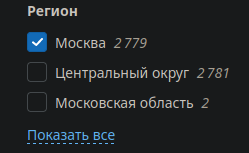
\includegraphics[scale=1]{fin2.png}}
	\caption{Количество вакансий в Москве}
	\label{fin2}
\end{figure}
\begin{figure}[H]
	\center{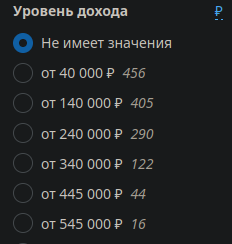
\includegraphics[scale=1]{fin1.png}}\
	\caption{Уровень дохода в Москве(из 2779 вакансий не у всех указан)}
	\label{fin1}
\end{figure}

\begin{figure}[H]
	\center{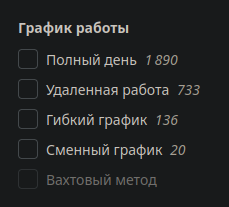
\includegraphics[scale=1]{fin3.png}}
	\caption{График работы в Москве}
	\label{fin3}
\end{figure}



% При использовании biblatex вместо bibtex
%\printbibliography

% Окончание основного документа и начало приложений Каждая последующая секция
% документа будет являться приложением
\end{document}
